\documentclass[dvipsnames]{report}
\usepackage[utf8]{inputenc}
\usepackage[dvipsnames]{xcolor}
\usepackage{tcolorbox}
\usepackage{multicol}
\usepackage{lipsum}
\usepackage[margin=0.4in]{geometry}
\usepackage{xstring}
\usepackage{xifthen}
\usepackage[dvipsnames]{xcolor}
\usepackage{setspace}
\usepackage{amsmath}
\usepackage{tabularx}
\pagenumbering{gobble}
\setlength{\columnsep}{1.5cm}
\setlength{\columnseprule}{0.2pt}
\usepackage{hyperref}
\usepackage[none]{hyphenat}
\hypersetup{
    colorlinks,
    citecolor=black,
    filecolor=black,
    linkcolor=black,
    urlcolor=black
}

\makeatletter
\def\@makechapterhead#1{%
  %\vspace*{5\p@}%
  {\parindent \z@ \raggedleft \normalfont
    \ifnum \c@secnumdepth >\m@ne
        \large\bfseries #1
%        \newline
        \par\nobreak
%        \vskip 10\p@
        \rule{\columnwidth}{.1pt}%
%        \vskip 10\p@
    \fi
    \interlinepenalty\@M
%    \large \bfseries \MakeUppercase{#1}\par\nobreak
%    \vskip 5\p@
  }}
\makeatother

\usepackage{enumitem}
\setitemize{noitemsep,topsep=0pt,parsep=0pt,partopsep=0pt}
\usepackage{graphicx}
\title{FF13-2 Any\%}
\author{MrTyton; desa3579}

\begin{document}
\singlespacing
\maketitle
\tableofcontents

\makeatletter
\patchcmd{\chapter}{\if@openright\cleardoublepage\else\clearpage\fi}{}{}{}
\makeatother

\newcommand{\syn}{\textbf{\textcolor{purple}{SYN}}}
\newcommand{\sab}{\textbf{\textcolor{gray}{SAB}}}
\newcommand{\com}{\textbf{\textcolor{red}{COM}}}
\newcommand{\rav}{\textbf{\textcolor{blue}{RAV}}}
\newcommand{\sen}{\textbf{\textcolor{BurntOrange}{SEN}}}
\newcommand{\med}{\textbf{\textcolor{green}{MED}}}
\newcommand{\gah}{\textbf{\textcolor{purple}{Gahongas}}}
\newcommand{\chu}{\textbf{\textcolor{red}{Chichu}}}
\newcommand{\nek}{\textbf{\textcolor{blue}{Nekton}}}
\newcommand{\X}{\textbf{X}}
\newcommand{\W}{\textbf{W}}
\newcommand{\nada}{\textbf{-}}
\newcommand{\comb}{\com-buffered into}

\newenvironment{battle}[1]{\begin{tcolorbox}[title=\begin{center}#1\end{center},colbacktitle=red!50!white]}{\end{tcolorbox}}

\newenvironment{shop}[1]{\begin{tcolorbox}[title=\begin{center}SHOP\, #1 GIL\end{center},colbacktitle=blue!50!white]}{\end{tcolorbox}}

\newenvironment{upgrade}{\begin{tcolorbox}[title=\begin{center}UPGRADE\end{center},colbacktitle=purple!50!white]}{\end{tcolorbox}}

\newenvironment{menu}{\begin{tcolorbox}[title=\begin{center}MENU\end{center},colbacktitle=black!50!white]}{\end{tcolorbox}}

\newcommand{\first}{1}
\newcommand{\second}{2}
\newcommand{\third}{3}
\newcommand{\fourth}{4}
\newcommand{\fifth}{5}
\newcommand{\sixth}{6}

\newcommand{\paradigm}{\item \textbf{Paradigm}}
\newcommand{\crystarium}{\item \textbf{Crystarium}}
\newcommand{\equip}{\item \textbf{Equipment}}
\newcommand{\skill}{\item \textbf{Fragment Skills}}


\newcommand{\stagger}{\textbf{STAGGER}}

\newcommand{\paradigmline}[5][]{\ifthenelse{\equal{#1}{}}{#2 & #3 & #4 & \ifthenelse{\equal{#5}{}}{\nada}{#5}}{#2 & #3 & #4 & \ifthenelse{\equal{#5}{}}{\nada}{\textit{#5}}& \textit{Default}}}


\newcommand{\paradigmdeck}[7]{\begin{tabularx}{.6\columnwidth}{c|c|c|XX} #1 \\ \cline{1-5} #2 \\ #3 \\ #4 \\ #5 \\ #6 \\ #7 \\ \end{tabularx}}

\newcommand{\paradigmdeckfour}[5]{\begin{tabular}{c|c|c|cc} #1 \\ \cline{1-4} #2 \\ #3 \\ #4 \\ #5 \\  \end{tabular}}

\newcommand{\stagebonus}[1]{Unlock the {#1} Stage Bonus}

\newcommand{\pickup}[2]{Pick up the \textbf{#1} located #2.}

\newcommand{\itemdrop}[2]{#1\% chance of a \textbf{#2}}

\newcommand{\throw}[2]{Throw Mog for \textbf{#1} located #2.}

\newcommand{\livet}[1]{Press {#1} on the Live Trigger}

\newcommand{\QTE}[1]{\textbf{Press {#1} on the QTE}}
\newcommand{\QTEE}[2]{\textbf{Press {#1}, then {#2} on the QTE}}
\newcommand{\QTEEE}[3]{\textbf{Press {#1}, then {#2} and {#3} on the QTE}}

\setlength{\columnsep}{.5cm}

\section*{Acknowledgements}
Everyone in the FF13 Discord. In no particular order: \textbf{Roostalol}, \textbf{LewdDolphin}, \textbf{Flux}, \textbf{Yeswally1}, \textbf{LilSharkie}, \textbf{xJakeDreamerx}, \textbf{TehMonkey\_},  \textbf{xP3ndulum},  \textbf{NijiBashira}, \textbf{Mrzwanzig}, \textbf{QazPlm9000}, \textbf{Hoishin}, \textbf{Tiornys}, \textbf{MLSTRM}, and anyone else I forgot.

\pagebreak


\begin{multicols}{2}
\chapter{Prologue}
\begin{enumerate}
	\item Press R3 three times when you have control of the camera.
	\item Talk to Basch, the guard, then open the gate.
	\item When you have control, open the menu
\end{enumerate}
\begin{menu}
	\begin{enumerate}
		\item Battle Mode: Active
		\item Battle Speed: 6
		\item Cursor Positon: Last Selection
	\end{enumerate}
\end{menu}
\begin{battle}{Air Cutter Remora}
	\begin{enumerate}
		\item Thunder x3 while runing in circles
		\item Alternate Attack-Thunder until out of MP
		\item Attack
	\end{enumerate}
\end{battle}
\begin{enumerate}
	\item Proceed up stairs, towards group, up stairs, up stairs.
\end{enumerate}
\begin{battle}{Imperial Guards}
	\begin{enumerate}
		\item Attack each guard twice
		\item Move towards exit while ATB is charging, then back to guards when full for Attack
	\end{enumerate}
\end{battle}
\chapter{Neo Bodhum 003AF}
\renewcommand{\first}{[1] Double Trouble (\com-\com)}
\renewcommand{\second}{[2] Slash \& Burn (\rav-\com)}
\renewcommand{\third}{[3] Misdirection (\com-\sen)}
\renewcommand{\fourth}{[4] Twin Shields (\sen-\sen)}
\renewcommand{\fifth}{[5] Dualcasting (\rav-\rav)}
\renewcommand{\sixth}{[6] Dualcasting (\rav-\rav)}
\begin{battle}{Nekton 1+1}
	\begin{itemize}
		\item \first
		      \begin{itemize}
			      \item Shift immediately
		      \end{itemize}
		\item \second
		      \begin{itemize}
			      \item Auto-Battle Meonekton
			      \item COM-Buffer last Fire
		      \end{itemize}
		\item \first
		      \begin{itemize}
			      \item Ruin x3 on Nekton while Noel finishes Meonekton
		      \end{itemize}
	\end{itemize}
\end{battle}
\begin{battle}{Nekton 1+3}
	\begin{itemize}
		\item \first
		      \begin{itemize}
			      \item Shift immediately
		      \end{itemize}
		\item \second
		      \begin{itemize}
			      \item Auto-Battle Meonekton
			      \item COM-Buffer last Fire
		      \end{itemize}
		\item \first
		      \begin{itemize}
			      \item Shift immediately
		      \end{itemize}
		\item \second
		      \begin{itemize}
			      \item Auto-Battle another Meonekton
			      \item COM-Buffer last Fire
		      \end{itemize}
		\item \first
		      \begin{itemize}
			      \item Ruin x3
		      \end{itemize}
		\item \second
		      \begin{itemize}
			      \item Auto-Battle the last Meonekton
			      \item Shift once Noel finished
		      \end{itemize}
		\item \first
		      \begin{itemize}
			      \item Repeat 2 Ruins
			      \item Noel should defeat the Nekton
		      \end{itemize}
	\end{itemize}
\end{battle}
\begin{battle}{Nekton 4+1}
	\begin{itemize}
		\item \first
		      \begin{itemize}
			      \item Ruin x3 on a Nekton
		      \end{itemize}
		\item \second
		      \begin{itemize}
			      \item Auto-Battle Meonekton
			      \item COM-Buffer last Fire
		      \end{itemize}
		\item \first
		      \begin{itemize}
			      \item Ruin x3 on a Nekton
			      \item \textbf{\textit{Cancel Noel}}
		      \end{itemize}
		\item \second
		      \begin{itemize}
			      \item Auto-Battle on Meonekton
		      \end{itemize}
	\end{itemize}
\end{battle}
\begin{battle}{Nekton 3+1}
	\begin{itemize}
		\item \first
		      \begin{itemize}
			      \item Ruin x3 on a Nekton
		      \end{itemize}
		\item \second
		      \begin{itemize}
			      \item Auto-Battle Meonekton
			      \item COM-Buffer last Fire
		      \end{itemize}
		\item \first
		      \begin{itemize}
			      \item Ruin x2
		      \end{itemize}
	\end{itemize}
\end{battle}

\pickup{Librascope}{After the slope behind the second Live Trigger}

\pickup{Phoenix Down}{After the third Live Trigger}

\begin{battle}{Gogmagog Alpha}
	\begin{itemize}
		\item \first
		      \begin{itemize}
			      \item Shift immediately
		      \end{itemize}
		\item \second
		      \begin{itemize}
			      \item Auto-Battle
		      \end{itemize}
		\item \first
		      \begin{itemize}
			      \item Shift immediately
		      \end{itemize}
		\item \second
		      \begin{itemize}
			      \item Auto-Battle
			      \item Repeat pattern until \stagger
		      \end{itemize}
		\item \first
		      \begin{itemize}
			      \item Ruin x2
		      \end{itemize}
		\item \second
		      \begin{itemize}
			      \item Fire x2
		      \end{itemize}
		\item \first
		      \begin{itemize}
			      \item Ruin x3 until you win
		      \end{itemize}
	\end{itemize}
\end{battle}

\pickup{300Gil}{Right after the Battle}

\pickup{Gysahl Green}{After the first jump on the left}

\begin{menu}
	\begin{itemize}
		\crystarium
		\begin{itemize}
			\item Serah
			      \begin{itemize}
				      \item All \rav
			      \end{itemize}
			\item Noel
			      \begin{itemize}
				      \item \rav Lv4
				      \item \textit{If you accidently activate \rav\ Lv5 you might as well go for all of them now}
			      \end{itemize}
		\end{itemize}
		\paradigm
		\begin{itemize}
			\item \paradigmdeck{%
				      \paradigmline{Serah}{Noel}{}{Orientation}}%
			      {\paradigmline[1]{\textit{\com}}{\textit{\com}}{}{\X}}%
			      {\paradigmline{\textit{\com}}{\com}{}{\X}}%
			      {\paradigmline{\com}{\textit{\rav}}{}{\W}}%
			      {\paradigmline{\sen}{\sen}{}{\W}}%
			      {\paradigmline{\textit{[\rav]}}{\textit{\rav}}{}{\W}}%
			      {\paradigmline{\textit{[\rav]}}{\textit{\rav}}{}{\W}}
		\end{itemize}
	\end{itemize}
\end{menu}

\livet{X}

\livet{Triangle}

\pickup{Phoenix Down}{Right before Gogmagog}

\renewcommand{\second}{[2] Double Trouble {(\com-\com)}}
\renewcommand{\third}{[3] Slash \& Burn{(\com-\rav)}}
\begin{battle}{Gogmagog Beta}
	\begin{itemize}
		\item \first
		      \begin{itemize}
			      \item Ruin x3
		      \end{itemize}
		\item \sixth
		      \begin{itemize}
			      \item Fire-Thunder-Fire
			      \item Repeat
		      \end{itemize}
		\item \fifth
		      \begin{itemize}
			      \item Repeat \stagger
			      \item Repeat
		      \end{itemize}
		\item \first
		      \begin{itemize}
			      \item Repeat
		      \end{itemize}
		\item \second
		      \begin{itemize}
			      \item Repeat until victory
		      \end{itemize}
	\end{itemize}
\end{battle}

\begin{menu}
	\begin{itemize}
		\crystarium
		\begin{itemize}
			\item Serah
			      \begin{itemize}
				      \item All RAV
			      \end{itemize}
			\item Noel
			      \begin{itemize}
				      \item All RAV
			      \end{itemize}
		\end{itemize}
	\end{itemize}
\end{menu}

\livet{Triangle}
\newline
\chapter{Bresha Ruins 005AF}

\begin{battle}{Paradox Alpha}
	\begin{itemize}
		\item \first
		      \begin{itemize}
			      \item Ruin x3
			      \item \textbf{\textit{Cancel Noel}}
		      \end{itemize}
		\item \second
		      \begin{itemize}
			      \item Repeat x2
			      \item \textbf{\textit{Cancel Noel}}
		      \end{itemize}
		\item \first
		      \begin{itemize}
			      \item Repeat
			      \item Ruin x2
			      \item \QTE{Right}
			      \item Repeat
		      \end{itemize}
		\item \second
		      \begin{itemize}
			      \item Repeat
			      \item Ruin x2
			      \item \QTEEE{Right}{Up}{X}
			      \item Repeat
			      \item \textbf{\textit{Cancel Noel}}
		      \end{itemize}
		\item \first
		      \begin{itemize}
			      \item Repeat
			      \item \QTE{Triangle}
		      \end{itemize}
	\end{itemize}
	\itemdrop{10}{Magician's Mark}
\end{battle}

\begin{battle}{Monster Crystal Tutorial}
	\begin{itemize}
		\item \first
		      \begin{itemize}
			      \item Ruin x3 \textit{on Cait Sith}
		      \end{itemize}
		\item \second
		      \begin{itemize}
			      \item Repeat
			      \item Repeat \textit{on Zwerg}
			      \item Repeat
		      \end{itemize}
		\item \first
		      \begin{itemize}
			      \item Repeat
		      \end{itemize}
	\end{itemize}
\end{battle}

\begin{battle}{Nekton Farming}
	\begin{itemize}
		\item \first
		      \begin{itemize}
			      \item \textit{Let Noel defeat all but one Nekton}
			      \item \textit{Retry if you don't get any Nekton Drops}
			      \item \textit{End the fight early if you get a Nekton Drop}
		      \end{itemize}
	\end{itemize}
\end{battle}

\pickup{Wild Artefact}{Behind the soldier}

\pickup{Phoenix Down}{In front of Atlas after activating the machine}

\begin{shop}{4400 - 6100}
	Sell all Phoenix Downs - Reference the Table to see how many Ghysal Greens and Droplets to Buy.
	\begin{center}
		\begin{tabular}{c|c|c}
			\textbf{Sell} & \textbf{Buy} & \textbf{Buy} \\
			$PD$          & $Gysahl$     & $Droplets$   \\
			\hline
			6             & 8            & 25           \\
			7             & 9            & 25           \\
			8             & 9            & 30           \\
			9             & 9            & 25           \\
			10            & 9            & 30           \\
		\end{tabular}
	\end{center}

	If you got at least 9 Phoenix Downs, also buy a Magician's Mark if you didn't have one dropped before.
\end{shop}

Once you have the Nekton, have Shopped, and completed the puzzles:

\begin{menu}
	\begin{itemize}
		\paradigm
		\begin{itemize}
			\item Insert \nek

			\item \paradigmdeck{%
				      \paradigmline{Serah}{Noel}{Monster}{Orientation}}%
			      {\paradigmline{\com}{\com}{\nek}{\X}}%
			      {\paradigmline{\textit{\com}}{\com}{\nek}{\X}}%
			      {\paradigmline{\com}{\rav}{\nek}{\W}}%
			      {\paradigmline{\sen}{\sen}{\nek}{\W}}%
			      {\paradigmline{\rav}{\rav}{\nek}{\W}}%
			      {\paradigmline[6]{\textit{\rav}}{\textit{\rav}}{\textit{\nek}}{\W}}
		\end{itemize}
		\crystarium
		\begin{itemize}
			\item Serah
			      \begin{itemize}
				      \item All \rav
				      \item \stagebonus{ATB Segment}
			      \end{itemize}
			\item Noel
			      \begin{itemize}
				      \item All \rav
				      \item \stagebonus{ATB Segment}
			      \end{itemize}
			\item Nekton
			      \begin{itemize}
				      \item All Potent Droplets
				      \item \stagebonus{ATB Segment}
			      \end{itemize}
		\end{itemize}
	\end{itemize}

	If you have another Magician's Mark equip it on Serah
\end{menu}

\renewcommand{\first}{[1]Aggression-X(\com-\com-\nek)}
\renewcommand{\second}{[2] Aggression-X (\rav-\com-\nek)}
\renewcommand{\third}{[3] Relentless Assault-W (\com-\rav-\nek)}
\renewcommand{\fourth}{[4] Patient Probing-W (\sen-\sen-\nek)}
\renewcommand{\fifth}{[5] Tri-Disaster-W (\rav-\rav-\nek)}
\renewcommand{\sixth}{[6] Tri-Disaster-W (\rav-\rav-\nek)}
\begin{battle}{Atlas}
	\begin{itemize}
		\item \sixth
		      \begin{itemize}
			      \item Fire-Blizzard-Fire-Blizzard
			      \item \textbf{\textit{Cancel Nekton}}
		      \end{itemize}
		\item \fifth
		      \begin{itemize}
			      \item Repeat
			      \item \textit{Get interrupted}
			      \item Repeat
			      \item Repeat 2 spells \stagger
			      \item \textit{Sometimes you need a third spell if your Refreshes aren't on point}
		      \end{itemize}
		\item \sixth
		      \begin{itemize}
			      \item Repeat
			      \item Fire-Fira-Fire
		      \end{itemize}
		\item \fifth
		      \begin{itemize}
			      \item Repeat
			      \item \QTEE{Right}{X}
			      \item \textit{Fail the second QTE}
		      \end{itemize}
	\end{itemize}
\end{battle}

Reveal the Artefact, then get on the Chocobo

\pickup{2 Gysahl Greens}{right before the slope}

\pickup{the artefact}{behind the bars}
\newline
\chapter{New Bodhum 003AF}

\pickup{Graviton Core}{On the platform on the left path}

Grind an encounter and Crux out once you can.
\newline
\chapter{Bresha Ruins 005AF}

Take the Chocobo to the gate, jumping off the ramp to the closed off path of grass. \pickup{hidden Graviton Core}{corner of the grass patch}
If you bought 25 Power Droplets earlier, then \pickup{Power Droplets}{in the same patch of grass}
\newline
\chapter{Yaschas Massif 010AF}

\pickup{500 Gil}{right at the start}

\pickup{8 Mana Slivers}{to the right of the closed gate}

\pickup{Gysahl Greens}{around the platform with Unicorn Horn}

\pickup{540 Gil}{shortly before Chocolina}

\begin{shop}{2000}
	\begin{itemize}
		\item Buy
		      \begin{itemize}
			      \item Magician's Mark x2
		      \end{itemize}
	\end{itemize}
\end{shop}

\begin{menu}
	\begin{itemize}
		\paradigm
		\begin{itemize}
			\item \paradigmdeck{%
				      \paradigmline{Serah}{Noel}{Monster}{Orientation}}%
			      {\paradigmline{\com}{\com}{\nek}{\X}}%
			      {\paradigmline{\textit{\com}}{\com}{\nek}{\textit{\W}}}%
			      {\paradigmline[3]{\textit{\com}}{\textit{\rav}}{\textit{\nek}}{\textit{\W}}}%
			      {\paradigmline{\sen}{\sen}{\nek}{\W}}%
			      {\paradigmline{\rav}{\rav}{\nek}{\W}}%
			      {\paradigmline{\rav}{\rav}{\nek}{\W}}
		\end{itemize}
		\crystarium
		\begin{itemize}
			\item Noel \& Serah
			      \begin{itemize}
				      \item All \rav
			      \end{itemize}
			\item Nekton
			      \begin{itemize}
				      \item All Mana Slivers
			      \end{itemize}
		\end{itemize}
		\equip
		\begin{itemize}
			\item Optimize Magic: Serah
			\item Optimize Magic: Noel
		\end{itemize}
		\item \textbf{Change Leader}
	\end{itemize}
\end{menu}

\renewcommand{\first}{[1]Aggression-X(\com-\com-\nek)}
\renewcommand{\second}{[2] Aggression-W (\com-\com-\nek)}
\renewcommand{\third}{[3] Relentless Assault-W (\rav-\com-\nek)}
\renewcommand{\fourth}{[4] Patient Probing-W (\sen-\sen-\nek)}
\renewcommand{\fifth}{[5] Tri-Disaster-W (\rav-\rav-\nek)}
\renewcommand{\sixth}{[6] Tri-Disaster-W (\rav-\rav-\nek)}
\begin{battle}{Aloeidai}
	\begin{flushleft}
		\begin{itemize}
			\item \textbf{Deprotega}
			      \begin{itemize}
				      \item \third
				            \begin{itemize}
					            \item Fire-Thunder-Fire-Thunder
					            \item \textit{Cancel Nekton}
				            \end{itemize}
				      \item \fifth
				            \begin{itemize}
					            \item Auto-Chain
					            \item \stagger\ cancel swipe
					            \item Bilzzara-Aerora
				            \end{itemize}
				      \item \sixth
				            \begin{itemize}
					            \item Repeat x2
					            \item ATB Refresh
				            \end{itemize}
				      \item \fifth
				            \begin{itemize}
					            \item Repeat
				            \end{itemize}
				      \item \second
				            \begin{itemize}
					            \item Ruin x4
					            \item ATB Refresh
				            \end{itemize}
				      \item \first
				            \begin{itemize}
					            \item Repeat
				            \end{itemize}
			      \end{itemize}
		\end{itemize}
		\begin{itemize}
			\item \textbf{Deshellga}
			      \begin{itemize}
				      \item \third
				            \begin{itemize}
					            \item Fire-Thunder-Fire-Thunder
					            \item \textit{Cancel Nekton}
				            \end{itemize}
				      \item \fifth
				            \begin{itemize}
					            \item Auto-Chain
					            \item \stagger\ cancel Ruinga
					            \item Blizzara-Aerora
				            \end{itemize}
				      \item \sixth
				            \begin{itemize}
					            \item Repeat
					            \item Potion through Ruinga
					            \item Repeat
					            \item ATB Refresh
				            \end{itemize}
				      \item \fifth
				            \begin{itemize}
					            \item Repeat
				            \end{itemize}
				      \item \fourth
				            \begin{itemize}
					            \item Tank Ruinga
				            \end{itemize}
				      \item \second
				            \begin{itemize}
					            \item Ruin x4
					            \item ATB Refresh
				            \end{itemize}
				      \item \first
				            \begin{itemize}
					            \item Repeat
				            \end{itemize}
			      \end{itemize}
		\end{itemize}
	\end{flushleft}
\end{battle}

\pickup{Gysahl Greens}{in the very back corner}

\livet{Triangle}

\pickup{Warding Talisman}{just before the stairs}

\begin{menu}
	\begin{itemize}
		\crystarium
		\begin{itemize}
			\item Noel
			      \begin{itemize}
				      \item All \rav
				      \item \stagebonus{ATB Segment}
			      \end{itemize}
			\item Serah
			      \begin{itemize}
				      \item \rav\ until Stagebonus
				      \item \stagebonus{\sab}
				      \item 2 \sab\ Levels (Deshell)
				      \item \rav\ until Level 47
			      \end{itemize}
		\end{itemize}
		\paradigm
		\begin{itemize}
			\item \paradigmdeck{%
				      \paradigmline{Noel}{Serah}{Monster}{Orientation}}%
			      {\paradigmline{\com}{\com}{\nek}{\X}}%
			      {\paradigmline{\com}{\com}{\nek}{\W}}%
			      {\paradigmline[3]{\textit{\rav}}{\textit{(\sab)}}{\textit{\nek}}{\textit{\W}}}%
			      {\paradigmline{\sen}{\sen}{\nek}{\W}}%
			      {\paradigmline{\rav}{\rav}{\nek}{\W}}%
			      {\paradigmline{\rav}{\rav}{\nek}{\W}}
		\end{itemize}
	\end{itemize}
\end{menu}

\renewcommand{\third}{[3] Smart Bomb-W (\rav/\sab/\nek)}
\begin{battle}{Gahongas}
	\begin{itemize}
		\item \third
		      \begin{itemize}
			      \item Auto-Battle Gahongas
			      \item Shift once Deshell hits
		      \end{itemize}
		\item \first
		      \begin{itemize}
			      \item Ruin x5
			      \item Repeat until Gahongas dies, then repeat the cycle on other Gahongas
			      \item \textit{If you don't tame Gahongas, retry the fight}
			      \item \textit{If you do tame Gahongas, defeat the others with the same method}
		      \end{itemize}
	\end{itemize}
\end{battle}

\begin{menu}
	\begin{itemize}
		\paradigm
		\begin{itemize}
			\item Insert Gahongas
			\item \paradigmdeck{%
				      \paradigmline{Noel}{Serah}{Monster}{Orientation}}%
			      {\paradigmline{\com}{\com}{\nek}{\X}}%
			      {\paradigmline{(\rav)}{(\rav)}{(\gah)}{\W}}%
			      {\paradigmline{\rav}{\sab}{\nek}{\W}}%
			      {\paradigmline{\sen}{\sen}{\nek}{\W}}%
			      {\paradigmline{\rav}{\rav}{\nek}{\W}}%
			      {\paradigmline[6]{\textit{\rav}}{\textit{\rav}}{\textit{\nek}}{\textit{\W}}}
		\end{itemize}
		\crystarium
		\begin{itemize}
			\item Gahongas
			      \begin{itemize}
				      \item Hit Level 6 for Faith
			      \end{itemize}
			\item Nekton
			      \begin{itemize}
				      \item Get Thunder if possible
			      \end{itemize}
		\end{itemize}
	\end{itemize}
\end{menu}
\chapter{Sunleth Waterscape 300AF}

\renewcommand{\second}{[2] Malevolence-W (\rav-\rav-\gah)}
\begin{battle}{Royal Ripeness}
	\begin{itemize}
		\item \sixth
		      \begin{itemize}
			      \item Aerora-Aero-Aerora
		      \end{itemize}
		\item \third
		      \begin{itemize}
			      \item Repeat
		      \end{itemize}
		\item \second
		      \begin{itemize}
			      \item Repeat
		      \end{itemize}
		\item \sixth
		      \begin{itemize}
			      \item COM-Buffer Aerora-Aerora
		      \end{itemize}
		\item \first
		      \begin{itemize}
			      \item Use Ruins if QTE didn't start
			      \item \QTE{[]}
			      \item Shift after QTE
		      \end{itemize}
		\item \sixth
		      \begin{itemize}
			      \item COM-Buffer Aerora-Aerora until victory
		      \end{itemize}
		\item \textbf{Press Up, followed by [], [], O and then right on the QTE}
	\end{itemize}
\end{battle}

\pickup{625 Gil}{on the left side before the first vine}

\begin{battle}{Miniflans 1}
	\begin{itemize}
		\item \sixth
		      \begin{itemize}
			      \item Shift immediately
		      \end{itemize}
		\item \second
		      \begin{itemize}
			      \item COM-Buffer Aerora x2
		      \end{itemize}
		\item \first
		      \begin{itemize}
			      \item Shift immediately
		      \end{itemize}
		\item \sixth
		      \begin{itemize}
			      \item Repeat pattern until you win
		      \end{itemize}
	\end{itemize}
\end{battle}
\chapter{Colosseum ???AF}

Skip 2 cutscenes, then Crux out.
\newline
\chapter{Sunleth Waterscape 300AF}

Run back and pawn an encounter before heading towards the vine.

\throw{7 Vitality Chips}{next to Chocolina}

\throw{960 Gil}{behind the second set of flans}

\begin{battle}{Miniflans 2}
	\begin{itemize}
		\item \sixth
		      \begin{itemize}
			      \item Shift immediately
		      \end{itemize}
		\item \second
		      \begin{itemize}
			      \item COM-Buffer Aerora x2
		      \end{itemize}
		\item \first
		      \begin{itemize}
			      \item Shift immediately
		      \end{itemize}
		\item \sixth
		      \begin{itemize}
			      \item Repeat pattern until you win
		      \end{itemize}
	\end{itemize}
\end{battle}

Take the Chocobo and head to the gate.
\newline
\chapter{Archlyte Steppe ???AF}
\pickup{Grimoire Hat}{on the platform}

\throw{600 Gil}{next to the stairs}

\begin{menu}
	\begin{itemize}
		\crystarium
		\begin{itemize}
			\item Noel \& Serah
			      \begin{itemize}
				      \item All \rav
			      \end{itemize}
		\end{itemize}
		\item {\textit{Continue only if Nekton doesn't have Thunder yet}}
		\item \textbf{Do either:}
		      \begin{itemize}
			      \crystarium
			      \begin{itemize}
				      \item Nekton
				            \begin{itemize}
					            \item Get Thunder
				            \end{itemize}
			      \end{itemize}
		      \end{itemize}
		\item \textbf{or:}
		      \begin{itemize}
			      \crystarium
			      \begin{itemize}
				      \item Zwerg Scandroid
				            \begin{itemize}
					            \item Get Thunder
				            \end{itemize}
			      \end{itemize}
			      \item \textbf{Monsters}
			            \begin{itemize}
				            \item Infuse Zwerg Scandroid into Nekton
			            \end{itemize}
		      \end{itemize}
	\end{itemize}
\end{menu}

\begin{battle}{Goblin Fragment}
	\begin{itemize}
		\item \sixth
		      \begin{itemize}
			      \item Blizzara-Blizzaga
		      \end{itemize}
		\item \third
		      \begin{itemize}
			      \item Repeat on Chocobo after Deshell
		      \end{itemize}
		\item \second
		      \begin{itemize}
			      \item Repeat, \com-buffer into
		      \end{itemize}
		\item \first
		      \begin{itemize}
			      \item Shift
		      \end{itemize}
		\item \textit{Until only the Flan is left:}
		      \begin{itemize}
			      \item \sixth
			            \begin{itemize}
				            \item Repeat, \com-buffer into
			            \end{itemize}
			      \item \first
			            \begin{itemize}
				            \item Shift
			            \end{itemize}
		      \end{itemize}
		\item \sixth
		      \begin{itemize}
			      \item Aerora-Aerora, \com-buffer into
		      \end{itemize}
		\item \first
		      \begin{itemize}
			      \item Repeat above as needed
		      \end{itemize}
	\end{itemize}
\end{battle}

Take the Cactuar to teleport back to camp. Throw mog to lure the sheep. After getting them all, for the weather: turn the left switch, then use the right one twice. Force a spawn before Faeryl.

\begin{battle}{Faeryl}
	\begin{itemize}
		\item \sixth
		      \begin{itemize}
			      \item Froststrike-SparkStrike-Froststrike- SparkStrike-Froststrike
		      \end{itemize}
		\item \fifth
		      \begin{itemize}
			      \item Repeat
			      \item Shift on \textbf{Megaton Charge}
		      \end{itemize}
		\item \fourth
		      \begin{itemize}
			      \item Tank it
		      \end{itemize}
		\item \second
		      \begin{itemize}
			      \item Wait until Faith
		      \end{itemize}
		\item \fourth
		      \begin{itemize}
			      \item Tank 3 hits of Quake
		      \end{itemize}
		\item \textit{Repeat Until Victory:}
		      \begin{itemize}
			      \item \sixth
			            \begin{itemize}
				            \item Potion if needed
				            \item Blizzara-Blizzaga, \com-buffer into
			            \end{itemize}
			      \item \first
			            \begin{itemize}
				            \item Shift
			            \end{itemize}
		      \end{itemize}
	\end{itemize}
\end{battle}

\throw{8 Power Slivers}{behind Faeryl}

Crux out in front of the \chu\ flower patch.
\chapter{Sunleth Waterscape 300AF}

Take the Chocobo if you bought at least 9 Ghystal Greens and haven't wasted any.

\begin{menu}
	\begin{itemize}
		\crystarium
		\begin{itemize}
			\item Noel
			      \begin{itemize}
				      \item All \rav
				      \item \stagebonus{\rav}
			      \end{itemize}
			\item Serah
			      \begin{itemize}
				      \item All \rav
				      \item \stagebonus{\sab}
			      \end{itemize}
		\end{itemize}
	\end{itemize}
\end{menu}

\begin{battle}{Mutantomato}
	\begin{itemize}
		\item \sixth
		      \begin{itemize}
			      \item Aerora-Aero-Aerora
		      \end{itemize}
		\item \third
		      \begin{itemize}
			      \item Repeat
		      \end{itemize}
		\item \second
		      \begin{itemize}
			      \item Repeat
		      \end{itemize}
		\item \sixth
		      \begin{itemize}
			      \item Repeat x2
		      \end{itemize}
		\item \fifth
		      \begin{itemize}
			      \item Repeat, \com-buffer into
		      \end{itemize}
		\item \first
	\end{itemize}
\end{battle}

\throw{Artefact}{on the yellow exclamation mark}
\newline

\chapter{Oerba 200AF}

%This shoudl all be done with actual figures

Anomaly 1 - Stage 1

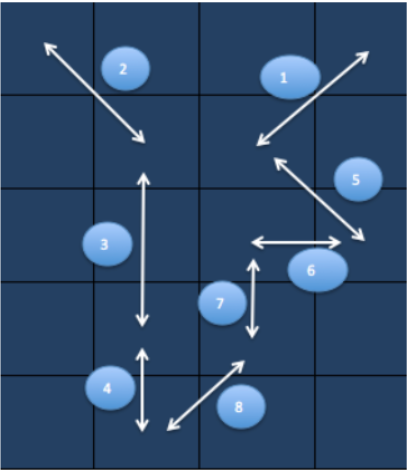
\includegraphics{Images/anomaly1stage1}

\pickup{2 Ghysal Greens}{if possible}

Anomaly 2 - Stage 1

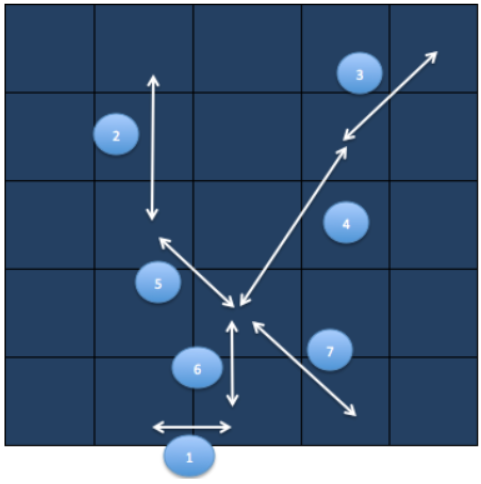
\includegraphics{Images/anomaly2stage1}

Anomaly 2 - Stage 2

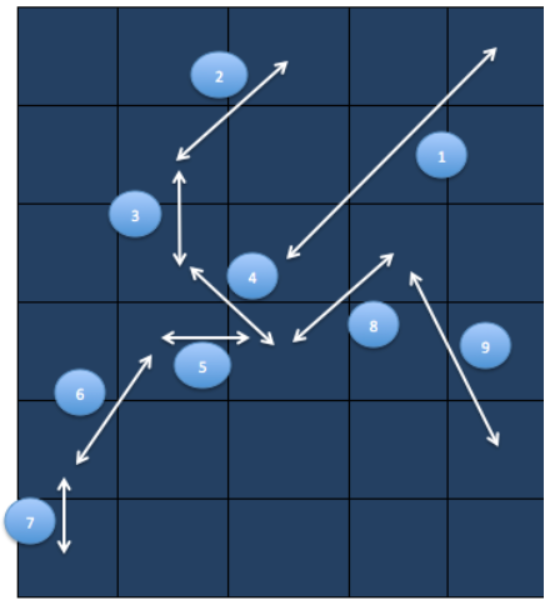
\includegraphics{Images/anomaly2stage2}

\pickup{500 Gil}{near the tree}

Anomaly 3 - Stage 1

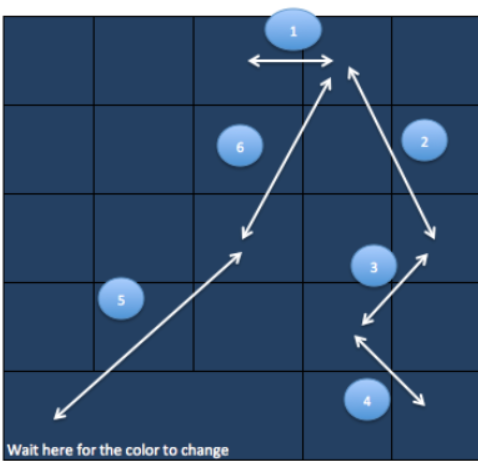
\includegraphics{Images/anomaly3stage1}

Anomaly 3 - Stage 2

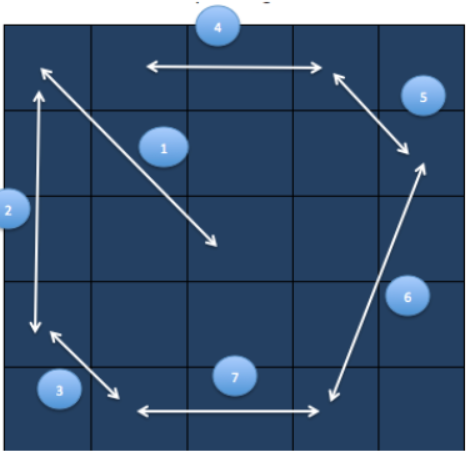
\includegraphics{Images/anomaly3stage2}

Anomaly 3 - Stage 3

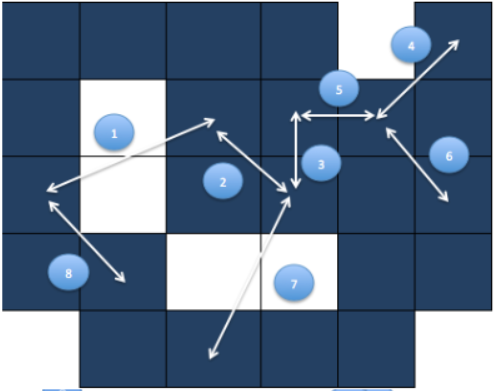
\includegraphics{images/anomaly3stage3}

\begin{menu}
	\begin{itemize}
		\crystarium
		\begin{itemize}
			\item Noel:
			      \begin{itemize}
				      \item All \rav
				      \item \stagebonus{\rav}
			      \end{itemize}
			\item Serah:
			      \begin{itemize}
				      \item All \rav
				      \item \stagebonus{ATB Level}
			      \end{itemize}
		\end{itemize}
	\end{itemize}
\end{menu}

\pickup{Librascope}{at the stairs}

\pickup{600 Gil}{in the house}

\begin{battle}{Oerba Caius}
	\begin{itemize}
		\item \sixth
		      \begin{itemize}
			      \item Shift
		      \end{itemize}
		\item \second
		      \begin{itemize}
			      \item Auto-Chain
			      \item Gahongas Feral Link
		      \end{itemize}
		\item \third
		      \begin{itemize}
			      \item Auto-Chain
		      \end{itemize}
		\item \fifth
		      \begin{itemize}
			      \item Blizzara-Aerora
			      \item Repeat, \com-buffer into
		      \end{itemize}
		\item \first
		      \begin{itemize}
			      \item Ruins x dead
		      \end{itemize}
	\end{itemize}
\end{battle}

Use the bathroom. Get the Ghysal Greens and Librascope if you haven't already. \pickup{Graviton Core}{on the building}. Head to the gate with the Chocobo.
\chapter{Yaschas Massif 01XAF}

Force an encounter near the rock where you farmed the Gahongas. Reveal and grab the Mysterious Artefact on the top of the stairs. Take the 600 Gil if you accidentally reveal it. Use the Chocobo, \pickup{Unicorn Horn}{up the stone ledge before the wide area} Get the 960 Gil chest if you haven't already while heading to the gate.
\newline

\chapter{Augusta Tower 300AF}

Throw Mog for the 9 Mana Slivers located to the left of the first room.

Retry and Crux Out if an Orion catches you.

Trigger the switch, then the next switch, then the next switch twice. After the elevator, two switches, then the next switch inside the room twice, then after the next elevator go through the room for the switch and trigger it three times. Force an encounter, trigger two switches, examine the computer.

\livet{\squarec}

Crux out.
\newline
\chapter{Yaschas Massif 01XAF}

Take the Chocobo.

\throw{10 Power Chips Chest}{at the chest}

Use the gate.
\newline

\chapter{Void Beyond ??? AF}

\throw{6 Potent Chips}{somewhere} Leave.
\newline
\chapter{Serendipity ???AF}

Unlock the Fragment Skills.

\begin{menu}
	\begin{itemize}
		\item \textbf{Fragment Skills:}
		      \begin{itemize}
			      \item Turn on both skills
		      \end{itemize}
	\end{itemize}
\end{menu}

Crux out.
\newline
\chapter{Archlyte Steppe ???AF}

\throw{Chichu}{in the flower patch} Do it again if you get the Super Hat.
\newline
\chapter{Academia 400F}

\begin{battle}{Ghouls}
  \begin{itemize}
    \item \sixth
          \begin{itemize}
            \item Auto-Chain, \com-buffer the first spell
          \end{itemize}
    \item \first
  \end{itemize}
\end{battle}

\begin{shop}{0}
  \begin{itemize}
    \item Sell:
          \begin{itemize}
            \item Everything but the \textit{Grimoire Hat}
          \end{itemize}
    \item Buy:
          \begin{itemize}
            \item 24 Power Slivers
          \end{itemize}
  \end{itemize}
\end{shop}

\begin{battle}{Koboldroid Yang x3}
  \begin{itemize}
    \item \textit{While there's more than 1 left:}
          \begin{itemize}
            \item \sixth
                  \begin{itemize}
                    \item Blizzara-Blizzaga, \com-buffer into
                  \end{itemize}
            \item \first
                  \begin{itemize}
                    \item Shift
                  \end{itemize}
          \end{itemize}
    \item \first
          \begin{itemize}
            \item Ruins x dead
          \end{itemize}
  \end{itemize}
\end{battle}

\begin{battle}{Fencer}
  \begin{itemize}
    \item \sixth
          \begin{itemize}
            \item Thunder x5
          \end{itemize}
    \item \fifth
          \begin{itemize}
            \item Repeat, \com-buffer into
          \end{itemize}
    \item \first
  \end{itemize}
\end{battle}

\begin{battle}{Taxim+Ghoul}
  \begin{itemize}
    \item \sixth
          \begin{itemize}
            \item Blizzara-Blizzaga
          \end{itemize}
    \item \fifth
          \begin{itemize}
            \item Repeat, \com-buffer into
          \end{itemize}
    \item \first
          \begin{itemize}
            \item Ruins if not dead
          \end{itemize}
  \end{itemize}
\end{battle}

\throw{8 Power Orbs}{somewhere}

Once you get to the 2 Taxim + 2 Nelapsis encounter, hit the furthest Taxim possible, retry, and continue running.

\throw{Kaiser Knuckes}{somewhere}

\begin{menu}
  \begin{itemize}
    \paradigm
    \begin{itemize}
      \item Replace \nek\ with \chu
    \end{itemize}
    \crystarium
    \begin{itemize}
      \item Chichu:
            \begin{itemize}
              \item All Power Silvers
              \item \stagebonus{ATB}
              \item All Potent Orbs
              \item All Power Orbs
            \end{itemize}
      \item Miniflan
            \begin{itemize}
              \item Level 3 if you have 6 Potent Orbs
            \end{itemize}
    \end{itemize}
    \item \textbf{Monsters}
          \begin{itemize}
            \item Infuse Nekton, Miniflan, or Gandayaks into Chichu
          \end{itemize}
  \end{itemize}
\end{menu}

\renewcommand{\first}{[1] Cerberus-X (\com-\com-\chu)}
\renewcommand{\third}{[3] Ruthless-W (\rav-\sab-\chu)}
\renewcommand{\fourth}{[4] Guarded Assault-W (\sen-\sen-\chu)}
\renewcommand{\fifth}{[5] Relentless Assault-W (\rav-\rav-\chu)}
\renewcommand{\sixth}{[6] Relentless Assault-W (\rav-\rav-\chu)}

\begin{battle}{Random Encounters}
  \begin{itemize}
    \item \sixth
          \begin{itemize}
            \item Shift
          \end{itemize}
    \item \second
          \begin{itemize}
            \item Blizzara-Blizzaga, \com-buffered into
          \end{itemize}
          \first
  \end{itemize}
\end{battle}

\pickup{Phoenix Down}{near encounters}

\begin{battle}{Cocytus + Nelapsi}
  \begin{flushleft}
    \begin{itemize}
      \item \sixth
            \begin{itemize}
              \item Shift
            \end{itemize}
      \item \second
            \begin{itemize}
              \item Aeroga-Aerora, \com-buffered into
            \end{itemize}
      \item \first
            \begin{itemize}
              \item Shift
            \end{itemize}
      \item \textit{Repeat until dead:}
            \begin{itemize}
              \item \sixth
                    \begin{itemize}
                      \item Aeroga-Aerora, \com-buffered into
                    \end{itemize}
              \item \first
                    \begin{itemize}
                      \item Shift
                    \end{itemize}
            \end{itemize}
    \end{itemize}
  \end{flushleft}
\end{battle}

\begin{battle}{Cocytus}
  \begin{flushleft}
    \begin{itemize}
      \item \sixth
            \begin{itemize}
              \item Shift
            \end{itemize}
      \item \second
            \begin{itemize}
              \item Aeroga-Aerora, \comb
            \end{itemize}
      \item \first
            \begin{itemize}
              \item Shift
            \end{itemize}
      \item \textit{Until Deshell:}
            \begin{itemize}
              \item \third
                    \begin{itemize}
                      \item Repeat, \comb
                    \end{itemize}
              \item \first
                    \begin{itemize}
                      \item Shift
                    \end{itemize}
            \end{itemize}
      \item \textit{Until Dead:}
            \begin{itemize}
              \item \sixth
                    \begin{itemize}
                      \item Repeat, \comb
                    \end{itemize}
              \item \first
                    \begin{itemize}
                      \item Shift
                    \end{itemize}
            \end{itemize}
    \end{itemize}
  \end{flushleft}
\end{battle}

\begin{battle}{Zenobia}
  \begin{flushleft}
    \begin{itemize}
      \item \sixth
            \begin{itemize}
              \item Auto-battle a tentacle
              \item Shift, canceling \chu
            \end{itemize}
      \item \fifth
            \begin{itemize}
              \item Auto-battle tentacles until they're dead
              \item Galestrike-Sparkstrike-Galestrike- Sparkstrike-Galestrike Zenoibia
            \end{itemize}
      \item \second
            \begin{itemize}
              \item Repeat
              \item Feral Link
            \end{itemize}
      \item \third
            \begin{itemize}
              \item Repeat, shift after Serah finishes debuffing
            \end{itemize}
      \item \fifth
            \begin{itemize}
              \item Aerora-Aero-Aerora once \stagger, maintain interruption
              \item Repeat, maintain interruption
              \item Shift when \chu\ will kill with enxt chain
            \end{itemize}
      \item \sixth
            \begin{itemize}
              \item Repeat as needed to kill
            \end{itemize}
    \end{itemize}
  \end{flushleft}
\end{battle}

\pickup{1050 Gil}{next to the gate if not done so yet}
\newline
\chapter{Augusta Tower 200AF}

\throw{Librascope}{the right after the room}
\throw{1500 Gil}{somewhere, if youy gil is low}
\livet{X}
\throw{Wild Artefact}{somewhere, before activating the bridge with the Keycard}

\begin{menu}
  \begin{itemize}
    \crystarium
    \begin{itemize}
      \item 1 \sab\ Level
      \item Max \rav
      \item \stagebonus{\sab}
    \end{itemize}
    \item Change Leader to Serah
  \end{itemize}
\end{menu}

\begin{battle}{Elevator 1}
  \begin{flushleft}
    \begin{itemize}
      \item \sixth
            \begin{itemize}
              \item Shift
            \end{itemize}
      \item \second
            \begin{itemize}
              \item Fira-Firaga, \comb
            \end{itemize}
      \item \first
            \begin{itemize}
              \item Shift
            \end{itemize}
      \item \textit{Repeat until dead:}
            \begin{itemize}
              \item \sixth
                    \begin{itemize}
                      \item Fira-Firaga Orion, \comb
                    \end{itemize}
              \item \first
                    \begin{itemize}
                      \item Shift
                    \end{itemize}
            \end{itemize}
    \end{itemize}
  \end{flushleft}
\end{battle}

\begin{battle}{Elevators 2+3}
  \begin{flushleft}
    \begin{itemize}
      \item \sixth
            \begin{itemize}
              \item Shift
            \end{itemize}
      \item \second
            \begin{itemize}
              \item Fira-Firaga, \comb
            \end{itemize}
      \item \first
            \begin{itemize}
              \item Shift
            \end{itemize}
      \item \textit{Repeat until dead:}
            \begin{itemize}
              \item \sixth
                    \begin{itemize}
                      \item Fira-Firaga \comb
                    \end{itemize}
              \item \first
                    \begin{itemize}
                      \item Shift
                    \end{itemize}
            \end{itemize}
    \end{itemize}
  \end{flushleft}
\end{battle}

\begin{menu}
  \begin{itemize}
    \crystarium
    \begin{itemize}
      \item Do one of the following:
            \begin{itemize}
              \item Orion: Level 13
              \item Dragoon: Level 18
            \end{itemize}
    \end{itemize}
    \item \textbf{Monsters}
          \begin{itemize}
            \item Infuse Orion/Dragoon into \chu, choose Adrenaline
          \end{itemize}
  \end{itemize}
\end{menu}

\throw{Magistral Chest}{52nd floor}
\pickup{8 Mana Engines}{between the second and third rooms}
\throw{8 Vitality Engines}{when walking back}
\throw{Gil Chests}{if your wallet is empty}

\begin{battle}{Feral Behemoth}
  \begin{flushleft}
    \begin{itemize}
      \item \sixth
            \begin{itemize}
              \item Shift
            \end{itemize}
      \item \second
            \begin{itemize}
              \item Auto-chain
              \item Feral Link
            \end{itemize}
      \item \third
            \begin{itemize}
              \item Deprotect x5
            \end{itemize}
      \item \fifth
            \begin{itemize}
              \item Auto-chain
            \end{itemize}
    \end{itemize}
  \end{flushleft}
\end{battle}

\begin{battle}{Proto Fal'Cie Adam 1}
  \begin{flushleft}
    \begin{itemize}
      \item \sixth
            \begin{itemize}
              \item Auto-chain
            \end{itemize}
      \item \fifth
            \begin{itemize}
              \item Auto-chain
            \end{itemize}
      \item \third
            \begin{itemize}
              \item Deprotect x5
            \end{itemize}
      \item \fifth
            \begin{itemize}
              \item Auto-chain
            \end{itemize}
    \end{itemize}
  \end{flushleft}
\end{battle}

\begin{battle}{Proto Fal'Cie Adam 2}
  \begin{flushleft}
    \begin{itemize}
      \item \sixth
            \begin{itemize}
              \item Librascope
              \item Thunder-Thundara-Thundara Right Manipulator
              \item Repeat on Left Manipulator once \chu\ attacks
              \item Shift after \chu\ kills the second Manipulator
            \end{itemize}
      \item \fifth
            \begin{itemize}
              \item Auto-chain, refresh with [6] until \stagger
            \end{itemize}
      \item \third
            \begin{itemize}
              \item Deprotect x3 \textit{if no Protect else} Deprotect x6-7
            \end{itemize}
      \item \fifth
            \begin{itemize}
              \item Repeat, refresh with [6] until dead
            \end{itemize}
    \end{itemize}
  \end{flushleft}
\end{battle}

Do not skip the second cutscene. \livet{[]}
\newline


\chapter{Academia 400F}
\pickup{Graviton Core}{bottom of the escalator after revealing it}
Jump back over the Phoenix Down chest to dodge an encounter, then go back to the gate on the bottom.
\newline
\chapter{Yaschas Massif 100AF}

Take the crazy chocobo, try making him face the way you want to go. Make sure to save a Ghysal Green and dismount before he eats it. \pickup{Graviton Core}{right side of the cliff} Crux out.
\newline
\chapter{Academia 4XXAF}

Turn in all Cores. \throw{Silver Chocobo}{somewhere}, talk to Noel. Take teh Chocobo and dismount at the game. \livet{Triangle}
\newline
\chapter{Void Beyond ??? AF}

\pickup{Librascope}{second or fourth Yuel}

\begin{battle}{Serah vs Caius}
	\begin{flushleft}
		\begin{itemize}
			\item \sixth
			      \begin{itemize}
				      \item Meteorite
				      \item Librascope
				      \item Auto-chain
			      \end{itemize}
			\item \fifth
			      \begin{itemize}
				      \item Auto-chain
			      \end{itemize}
		\end{itemize}
	\end{flushleft}
\end{battle}
\chapter{Dying World 700AF}

\begin{battle}{Noel vs Caius}
	\begin{itemize}
		\item Check the amount and order of your items
		\item Die
	\end{itemize}
\end{battle}

\pickup{8 Power Essences}{behind the wall on the right before the cutscene trigger}

\begin{battle}{Gogmagog Gamma}
	\begin{flushleft}
		\begin{itemize}
			\item \sixth
			      \begin{itemize}
				      \item Shift Immediately
			      \end{itemize}
			\item \second
			      \begin{itemize}
				      \item Auto-chain
				      \item Feral Link
			      \end{itemize}
			\item \third
			      \begin{itemize}
				      \item Auto-debuff
			      \end{itemize}
			\item \textit{Repeat 3 times:}
			      \begin{itemize}
				      \item \fifth
				            \begin{itemize}
					            \item Fira-Firaga, \comb
				            \end{itemize}
				      \item \first
				            \begin{itemize}
					            \item Shift
				            \end{itemize}
			      \end{itemize}
		\end{itemize}
	\end{flushleft}
\end{battle}

\pickup{10 Vitality Essences}{behind of the trees in the desert wasteland}
\newline
\chapter{New Bodhum 700AF}

Reveal the Artefact and grab it.
\newline
\chapter{Serendipity ???AF}

Unlock the Fragment Skills.

\begin{menu}
  \begin{itemize}
    \item \textbf{Fragment Skills:}
          \begin{itemize}
            \item Turn on everything
          \end{itemize}
    \item \textbf{Monsters}
          \begin{itemize}
            \item Influse Silver Chocobo into \chu
          \end{itemize}
  \end{itemize}
\end{menu}

Crux out.
\newline
\chapter{Academia 500F}

\begin{shop}{60000}
  \begin{itemize}
    \item Sell:
          \begin{itemize}
            \item Accessories:
                  \begin{itemize}
                    \item All but \textit{Grimoire Hat}
                  \end{itemize}
            \item Components:
                  \begin{itemize}
                    \item First Slot
                    \item Tears of Remorse
                    \item Gold Nuggets
                    \item Any Expensive Monster Materials \textit{Except Essences, Crystals, and Orbs}
                  \end{itemize}
          \end{itemize}
    \item Buy:
          \begin{itemize}
            \item Monster Materials:
                  \begin{itemize}
                    \item 16 Power Orbs
                    \item 32 Power Essences
                  \end{itemize}
            \item Items
                  \begin{itemize}
                    \item 21 Potions
                  \end{itemize}
          \end{itemize}
  \end{itemize}
\end{shop}
\begin{menu}
  \begin{itemize}
    \crystarium
    \begin{itemize}
      \item Noel
            \begin{itemize}
              \item \sen\ Level 40
              \item \stagebonus{Reprieve}
              \item \stagebonus{ACC Slot}
            \end{itemize}
      \item \chu
            \begin{itemize}
              \item If you only have 6 Potent Orbs, use them
              \item Power Orbs
              \item \stagebonus{ATB}
              \item Vitality Essences
              \item Power Essences
            \end{itemize}
    \end{itemize}
    \equip
    \begin{itemize}
      \item Noel: Grimoire Hat
    \end{itemize}
  \end{itemize}
\end{menu}

Go Left first, then turn Right towards the L-Block. Turn Right and jump onto the next L-Block.

\begin{battle}{Pacos Amethys and Pacos Luvulite}
  \begin{flushleft}
    \begin{itemize}
      \item \sixth
            \begin{itemize}
              \item Switch Target to Amethyst
              \item Librascope
              \item Flamestrike x5
            \end{itemize}
      \item \third
            \begin{itemize}
              \item Repeat
              \item Potion as needed
              \item Shift after Serah finishes her second chain on Luvulite
            \end{itemize}
      \item \fifth
            \begin{itemize}
              \item Repeat, ATB refresh with [6] until Amethyst dies
              \item Blizzard x5
              \item Hope that either Serah or Noel dies, Potion \chu\ to keep him in green hp
              \item Blizzara-Blizzaga when Split Starts
              \item Repeat and refresh with [6] until end
            \end{itemize}
    \end{itemize}
  \end{flushleft}
\end{battle}

Turn around and examine the switch. Turn Left, wait for the L-Block. Run back utnil the next switch, run back to the next L-Block. \throw{Shaman's Mark}{somewhere}

Once the L-Block rotates, go to the other side, then head east. Halfway through the long walk use the Cactuar. Once the T-Block faces north or west, use the switch. Jump on the T-Block and onto the stairs.

Jump on the stationary L-Block, then go for the next T-Block.

Go onto the next platform and waitf or the next T-Block. \throw{7 Vitality Boosters}{somewhere if your Gil is low}

Jump onto the next T-Block. If you got 2 Scarletites, wait for it to rotate twice, otherwise only once. Run up the stairs to the L-block and jump to stay on it when it turns.

After it's finished rotating, go to the new way and \throw{8 Mana Essences Chest}{on the platform}

Run to the other end of the L-block and make the jump to the L-block below.

\begin{battle}{Apkallu PRE-EMPT}
  \begin{flushleft}
    \begin{itemize}
      \item \sixth
            \begin{itemize}
              \item Thunder x5
            \end{itemize}
      \item \fifth
            \begin{itemize}
              \item Repeat x2
            \end{itemize}
    \end{itemize}
  \end{flushleft}
\end{battle}

Examine the switch. Run back to the L-block. Jump back to the T-block and go north. Turn Left and wait for the L-block to rotate. Go up the last set of stairs.

\begin{shop}{41000}
  \begin{itemize}
    \item Sell:
          \begin{itemize}
            \item Everything but Power Essences and Potent Crystals
          \end{itemize}
    \item Buy:
          \begin{itemize}
            \item 21 Power Essences
          \end{itemize}
  \end{itemize}
\end{shop}
\begin{menu}
  \begin{itemize}
    \crystarium
    \begin{itemize}
      \item \chu
            \begin{itemize}
              \item All Power Essences
              \item \stagebonus{ATB Segment}
              \item All Potent Crystals
            \end{itemize}
    \end{itemize}
  \end{itemize}
\end{menu}

\begin{battle}{Chaos Bahamut 3}
  \begin{flushleft}
    \begin{itemize}
      \item \sixth
            \begin{itemize}
              \item Auto-chain
              \item Shift after second swipe
            \end{itemize}
      \item \second
            \begin{itemize}
              \item Auto-chain
              \item Feral Link
            \end{itemize}
      \item \sixth
            \begin{itemize}
              \item Potion
              \item Auto-chain, refresh with [6] until Megaflare
            \end{itemize}
      \item \fourth
            \begin{itemize}
              \item Tank Megaflare
              \item Potion
            \end{itemize}
      \item \fifth
            \begin{itemize}
              \item Potion if \chu\ is not in green hp
              \item Repeat, refresh with [6] until dead
            \end{itemize}
    \end{itemize}
  \end{flushleft}
\end{battle}

\begin{battle}{Deck Caius}
  \begin{flushleft}
    \begin{itemize}
      \item \sixth
            \begin{itemize}
              \item Auto-chain
            \end{itemize}
      \item \fifth
            \begin{itemize}
              \item Auto-chain
              \item Fire-Thunder-Fire-Thunder
            \end{itemize}
      \item \sixth
            \begin{itemize}
              \item Repeat
            \end{itemize}
    \end{itemize}
  \end{flushleft}
\end{battle}

\begin{battle}{Beach Caius}
  \begin{flushleft}
    \begin{itemize}
      \item \sixth
            \begin{itemize}
              \item Aerora-Aero-Aerora, execute after Serah starts chaining
            \end{itemize}
      \item \fifth
            \begin{itemize}
              \item Aerora-Aero
            \end{itemize}
      \item \fourth
            \begin{itemize}
              \item Shift once Serah Provokes
            \end{itemize}
      \item \fifth
            \begin{itemize}
              \item \stagger\ once Serah is about to die or is dead
              \item Aerora-Aero-Aerora
            \end{itemize}
      \item \sixth
            \begin{itemize}
              \item Repeat
            \end{itemize}
    \end{itemize}
  \end{flushleft}
\end{battle}

\begin{battle}{Final Bahamut}
  \begin{flushleft}
    \begin{itemize}
      \item \sixth
            \begin{itemize}
              \item Librascope
            \end{itemize}
      \item \fifth
            \begin{itemize}
              \item Auto-chain Garnet
            \end{itemize}
      \item \third
            \begin{itemize}
              \item Auto-chain
            \end{itemize}
      \item \fifth
            \begin{itemize}
              \item Auto-chain
              \item Potion
              \item Auto-chain, refresh with [6] until Garnet dies
              \item Fire-Thunder-Fire-Thunder-Fire on Amber
            \end{itemize}
      \item \third
            \begin{itemize}
              \item Repeat
            \end{itemize}
      \item \fifth
            \begin{itemize}
              \item Repeat until Amber dies
              \item Make sure that you're at almost full HP
              \item Unicorn Horn after Break Curse
              \item Repeat
              \item Shift after the First Dark Flame
            \end{itemize}
      \item \second
            \begin{itemize}
              \item Repeat
              \item Feral Link
              \item Potion
            \end{itemize}
      \item \sixth
            \begin{itemize}
              \item Repeat
            \end{itemize}
      \item \third
            \begin{itemize}
              \item Repeat until Deprotect
            \end{itemize}
      \item \fifth
            \begin{itemize}
              \item Hope that Serah died
              \item Aerora-Aero-Aerora, repeat with [6] until dead
              \item If he uses any more moves, tank in \fourth
            \end{itemize}
    \end{itemize}
  \end{flushleft}
\end{battle}


\end{multicols}

\end{document}
